\documentclass[11pt]{article}
\usepackage[margin=1in]{geometry}
\usepackage{amsmath,amssymb,amsthm,mathtools}
\usepackage{graphicx}
\usepackage{hyperref}
\usepackage{xcolor}

\newtheorem{theorem}{Theorem}
\newtheorem{lemma}[theorem]{Lemma}
\newtheorem{proposition}[theorem]{Proposition}
\newtheorem{corollary}[theorem]{Corollary}
\newcommand{\Lip}{\operatorname{Lip}}
\newcommand{\R}{\mathbb R}
\newcommand{\G}{\Gamma}
\newcommand{\gLip}{\gamma^{\mathrm{Lip}}_2}
\newcommand{\Sig}{\Sigma}

\title{Metric Hilbert Factorization Does Not Imply\\
Multilinear Hilbert Factorization}
\author{Automatic mathematics run \texttt{fa\_banach\_001}}
\date{9 August 2026}

\begin{document}
\setlength{\emergencystretch}{3em}
\maketitle

\begin{center}
\fbox{\parbox{0.91\textwidth}{
\textbf{Status.} Candidate counterexample, likely valid, for human review.
The construction is over the real scalars.  It answers both Questions 1 and 2
in Section 2.2 of Fern\'andez-Unzueta--Garc\'ia-Hern\'andez negatively.
}}
\end{center}

\section{Source question}

The source is M. Fern\'andez-Unzueta and S. Garc\'ia-Hern\'andez,
\emph{Multilinear Operators Factoring through Hilbert Spaces},
arXiv:1805.09748, later published in \emph{Banach Journal of Mathematical
Analysis} 13 (2019), 234--254 \cite{source}.

For a multilinear operator
$T:X_1\times\cdots\times X_n\to Y$, the paper writes
$f_T:\Sig_{X_1,\ldots,X_n}^{\pi}\to Y$ for the restriction of the
linearization of $T$ to the Segre cone.  It proves
\[
  \gLip(f_T)\leq \G(T),
\]
where $\G(T)$ is the multilinear Hilbert-factorization norm and
$\gLip$ is the metric factorization norm through a subset of a Hilbert space.
The authors ask:

\begin{quote}
\textbf{Question 1.} Is the map $T\mapsto f_T$ an isometry?

\textbf{Question 2.} If $f_T$ factors through a Hilbert space in the metric
sense, must $T$ factor through a Hilbert space in the multilinear sense?
\end{quote}

The statement occurs across printed pages 7--8.  The two source crops are
included below.

\begin{center}
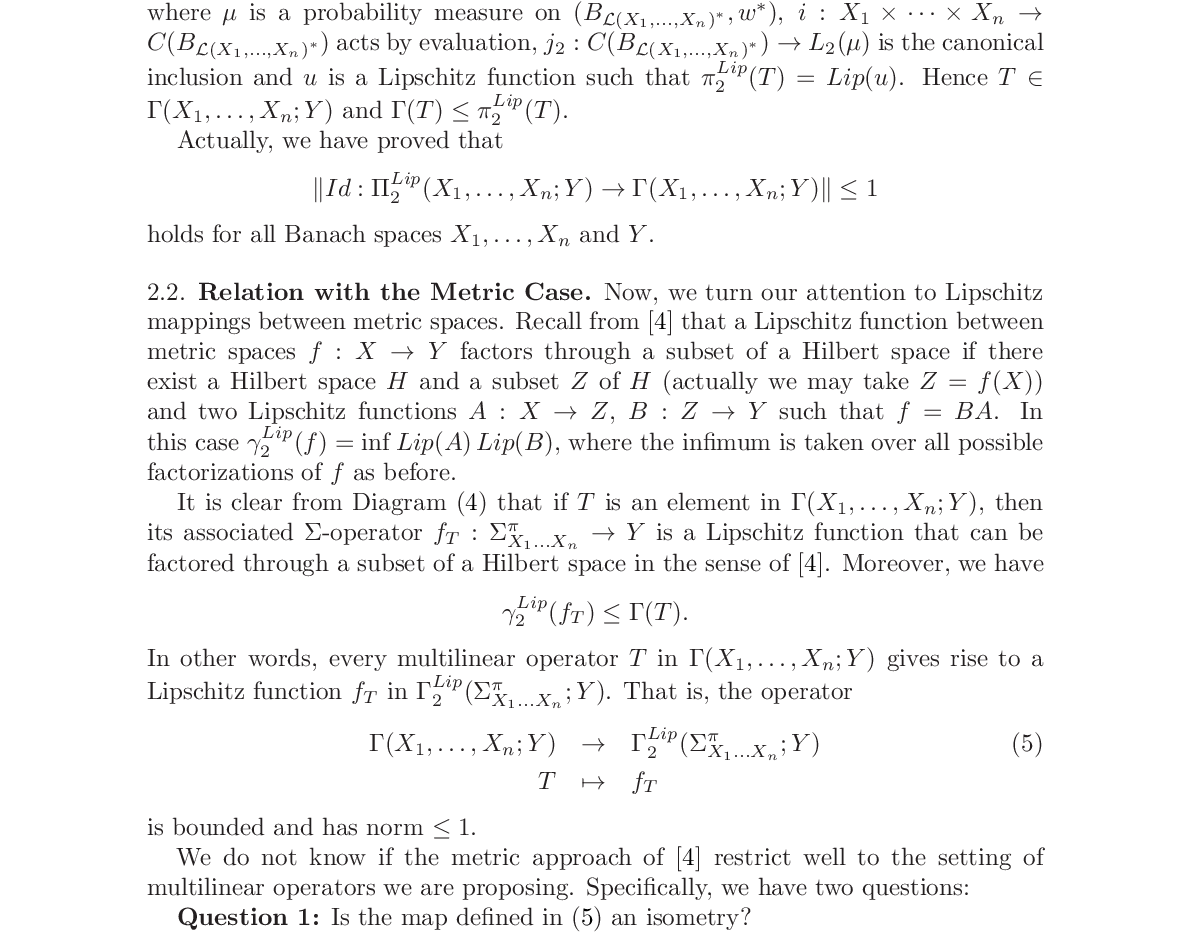
\includegraphics[width=0.96\textwidth]{figures/open_problem_crop_page7.png}

\medskip
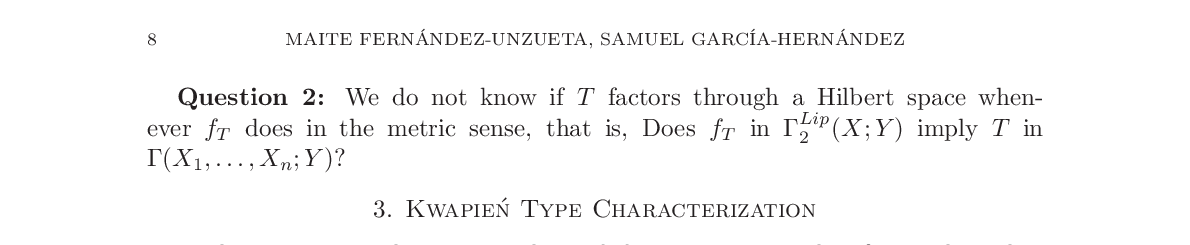
\includegraphics[width=0.96\textwidth]{figures/open_problem_crop_page8.png}
\end{center}

\section{Definitions used in the construction}

All spaces below are real.  If $S:X_1\times\cdots\times X_n\to Y$ is
multilinear, then $S\in\G(X_1,\ldots,X_n;Y)$ means that
\[
 S=B\circ A,
\]
where $A$ is a bounded multilinear map into a Hilbert space $H$, and $B$ is
Lipschitz on $A(X_1\times\cdots\times X_n)$.  The norm $\G(S)$ is the
infimum of $\|A\|\Lip(B)$.

For a Lipschitz map $f:M\to Y$, $\gLip(f)$ is the infimum of
$\Lip(a)\Lip(b)$ over factorizations $f=b\circ a$ with $a$ mapping $M$
into a subset of a Hilbert space and $b$ Lipschitz there.

Write $E_m=\ell_1^m$ and identify
\[
 E_m\widehat\otimes_\pi E_m=\ell_1^{m\times m}
\]
by the usual matrix coordinates.  Let
\[
 J_m:E_m\times E_m\longrightarrow \ell_1^{m\times m},
 \qquad J_m(x,y)=x\otimes y.
\]
Its associated Segre operator is the identity map on the rank-one cone
$\Sig_m=\{x\otimes y:x,y\in E_m\}$, equipped with the ambient entrywise
$\ell_1$ metric.

\section{Idea of the proof}

There are two different geometries in the source comparison.  A multilinear
factorization of $J_m$ must encode every sign tensor
$\varepsilon\otimes\delta$ by a \emph{bilinear} Hilbert-valued map.  A
Rademacher average then forces distortion at least $m$, and the elementary
coordinate embedding shows that the exact value is $\G(J_m)=m$.

The metric factor may encode the rank-one cone nonlinearly.  A nonzero
rank-one matrix has the form $r(u\otimes v)$, where $r$ is its $\ell_1$ norm
and $u,v$ are on the $\ell_1$ unit sphere, uniquely up to the simultaneous
sign change $(u,v)\mapsto(-u,-v)$.  The quadratic Hilbert feature
\[
 (u,v)\longmapsto
 \frac{(u,v)\otimes(u,v)}{\|(u,v)\|_2}
\]
removes exactly that sign ambiguity.  Its distortion on the direction space
is $O(\sqrt m)$; adjoining the radial coordinate preserves this order on the
whole cone.  Hence $\gLip(f_{J_m})=O(\sqrt m)$, strictly smaller than
$\G(J_m)=m$ for large $m$.

Finally, put increasingly large finite-dimensional examples on diagonal
blocks and weight the $m$th block by the reciprocal of its metric bound.  The
Segre map then has a metric Hilbert factorization with constant $1$, whereas
the multilinear $\G$-norms of the block restrictions tend to infinity.  This
produces one bounded bilinear operator outside $\G$ and answers Question 2.

\section{A Hilbert embedding of the rank-one cone}

Let
\[
 \mathcal R_m=\{u\otimes v:\|u\|_1=\|v\|_1=1\}\subset\Sig_m.
\]
For $a=u\otimes v$ and $b=u'\otimes v'$ in $\mathcal R_m$, put
\begin{align*}
 \rho(a,b)&=\|a-b\|_1,\\
 \delta(a,b)&=\min_{\sigma\in\{-1,1\}}
 \bigl(\|u-\sigma u'\|_1+\|v-\sigma v'\|_1\bigr).
\end{align*}

\begin{lemma}[Stability of normalized rank-one factors]\label{lem:direction}
For all $a,b\in\mathcal R_m$,
\[
 \rho(a,b)\leq\delta(a,b)\leq 8\rho(a,b).
\]
\end{lemma}

\begin{proof}
For either sign $\sigma$,
\[
 u\otimes v-u'\otimes v'
 =(u-\sigma u')\otimes v+\sigma u'\otimes(v-\sigma v'),
\]
so $\rho\leq\delta$.

Suppose first that $\rho<1/2$.  Choose $f\in B_{\ell_\infty^m}$ with
$f(u)=1$.  Contracting the first tensor coordinate gives
\[
 \|v-f(u')v'\|_1\leq\rho.
\]
Thus $|f(u')|\geq1-\rho>1/2$.  With
$\sigma=\operatorname{sign}f(u')$,
\[
 \|v-\sigma v'\|_1\leq2\rho.
\]
Choose $g\in B_{\ell_\infty^m}$ with $g(v)=1$.  Contracting the second
coordinate gives $\|u-g(v')u'\|_1\leq\rho$, while
\[
 |g(v')-\sigma|
 \leq\|v'-\sigma v\|_1\leq2\rho.
\]
Consequently $\|u-\sigma u'\|_1\leq3\rho$, so in fact
$\delta\leq5\rho$.  If $\rho\geq1/2$, the trivial bound
$\delta\leq4$ gives $\delta\leq8\rho$.
\end{proof}

For $a=u\otimes v\in\mathcal R_m$, set $w_a=(u,v)\in\R^{2m}$ and define
\[
 h_m(a)=\frac{w_a\otimes w_a}{\|w_a\|_2}
 \quad\text{in}\quad
 K_m:=\R^{2m}\widehat\otimes_2\R^{2m}.
\]
The map is well-defined because the only ambiguity in normalized real
rank-one factors is $(u,v)\mapsto(-u,-v)$.  Also
$\|h_m(a)\|_2=\|w_a\|_2\leq\sqrt2$.

\begin{lemma}[Quadratic quotient feature]\label{lem:quadratic}
For $a,b\in\mathcal R_m$,
\[
 \frac{\rho(a,b)}{\sqrt{2m}}
 \leq \|h_m(a)-h_m(b)\|_2
 \leq 8\sqrt2\,\rho(a,b).
\]
\end{lemma}

\begin{proof}
Let
\[
 d_2=\min_{\sigma\in\{-1,1\}}\|w_a-\sigma w_b\|_2.
\]
Write $\alpha=\|w_a\|_2$, $\beta=\|w_b\|_2$, and
$c=|\langle w_a,w_b\rangle|/(\alpha\beta)$.  Then
\begin{align*}
 d_2^2&=\alpha^2+\beta^2-2\alpha\beta c,\\
 \|h_m(a)-h_m(b)\|_2^2
 &=\alpha^2+\beta^2-2\alpha\beta c^2.
\end{align*}
Since
$2\alpha\beta(c-c^2)\leq2\alpha\beta(1-c)\leq d_2^2$,
\[
 d_2\leq\|h_m(a)-h_m(b)\|_2\leq\sqrt2\,d_2.
\]
Moreover,
\[
 d_2\leq\delta(a,b)\leq\sqrt{2m}\,d_2.
\]
Combine these inequalities with Lemma~\ref{lem:direction}.
\end{proof}

Every nonzero $p\in\Sig_m$ has a unique representation
$p=r a$, where $r=\|p\|_1>0$ and $a\in\mathcal R_m$.  Define
\[
 F_m(0)=0,
 \qquad
 F_m(ra)=\bigl(r,rh_m(a)\bigr)\in H_m:=\R\oplus_2 K_m.
\]

\begin{proposition}[Metric factorization bound]\label{prop:metric}
The map $F_m$ is bi-Lipschitz and
\[
 \Lip(F_m)\leq24\sqrt2,
 \qquad
 \Lip(F_m^{-1})\leq5\sqrt m.
\]
Consequently
\[
 \gLip(f_{J_m})\leq120\sqrt{2m}.
\]
\end{proposition}

\begin{proof}
Take $p=ra$ and $q=sb$ and suppose $r\geq s\geq0$.  Put
$d=\|p-q\|_1$ and $\rho=\rho(a,b)$ when $s>0$ (when $s=0$ the same
estimates follow directly).  The triangle inequality and its reverse give
\[
 r-s\leq d,
 \qquad
 s\rho\leq d+(r-s)\leq2d,
\]
hence
\[
 (r-s)+s\rho\leq3d,
 \qquad
 d\leq(r-s)+s\rho.                                      \tag{1}
\]
Let $D=\|F_m(p)-F_m(q)\|_2$.  By
Lemma~\ref{lem:quadratic} and $\|h_m(a)\|_2\leq\sqrt2$,
\begin{align*}
 D
 &\leq (r-s)+\|rh_m(a)-sh_m(b)\|_2\\
 &\leq(1+\sqrt2)(r-s)+8\sqrt2\,s\rho
 \leq24\sqrt2\,d,
\end{align*}
using (1).

Conversely, $r-s\leq D$, and
\[
 s\|h_m(a)-h_m(b)\|_2
 \leq\|rh_m(a)-sh_m(b)\|_2+(r-s)\|h_m(a)\|_2
 \leq(1+\sqrt2)D.
\]
Lemma~\ref{lem:quadratic} and (1) now imply
\[
 d\leq(r-s)+s\rho
 \leq\bigl[1+(1+\sqrt2)\sqrt{2m}\bigr]D
 \leq5\sqrt m\,D.
\]
Thus $F_m$ has the stated constants.  Since $f_{J_m}$ is the identity on
$\Sig_m$, the factorization $f_{J_m}=F_m^{-1}\circ F_m$ proves the final
bound.
\end{proof}

\section{The exact multilinear norm}

\begin{proposition}\label{prop:gamma}
For every $m\geq1$,
\[
 \G(J_m)=m.
\]
\end{proposition}

\begin{proof}
For the upper bound, regard
$A(x,y)=x\otimes y$ as taking values in the Hilbert space
$\ell_2^{m\times m}$.  Then $\|A\|=1$.  On the rank-one cone, let $B$ be
the identity into $\ell_1^{m\times m}$.  Since
$\|z\|_1\leq m\|z\|_2$ for every $z\in\R^{m\times m}$,
$\Lip(B)\leq m$.  Hence $\G(J_m)\leq m$.

For the reverse inequality, let $J_m=B\circ A$ be any multilinear Hilbert
factorization, and set $a_{ij}=A(e_i,e_j)$.  For independent Rademacher
vectors $\varepsilon,\delta\in\{-1,1\}^m$, orthogonality gives
\[
 \mathbb E\|A(\varepsilon,\delta)\|_2^2
 =\sum_{i,j=1}^m\|a_{ij}\|_2^2
 \leq m^2\|A\|^2.
\]
Thus some sign pair satisfies
$\|A(\varepsilon,\delta)\|_2\leq m\|A\|$.  As
$A(0,\delta)=0$ and
$\|J_m(\varepsilon,\delta)\|_1=m^2$,
\[
 m^2
 \leq\Lip(B)\|A(\varepsilon,\delta)\|_2
 \leq m\|A\|\Lip(B).
\]
Taking the infimum gives $\G(J_m)\geq m$.
\end{proof}

\begin{corollary}[Negative answer to Question 1]\label{cor:q1}
The comparison $T\mapsto f_T$ is not an isometry.  In fact, for
$m=2^{15}=32768$,
\[
 \gLip(f_{J_m})\leq120\sqrt{2m}=30720
 <32768=\G(J_m).
\]
Moreover, the ratio $\G(J_m)/\gLip(f_{J_m})$ is unbounded as $m\to\infty$.
\end{corollary}

\section{A single operator outside the multilinear ideal}

Choose any sequence $m_k\to\infty$ and put
\[
 c_k=120\sqrt{2m_k},
 \qquad
 \omega_k=c_k^{-1}.
\]
Let
\[
 X=\left(\bigoplus_{k=1}^\infty E_{m_k}\right)_{\ell_1},
 \qquad
 Z=\left(\bigoplus_{k=1}^\infty
          \ell_1^{m_k\times m_k}\right)_{\ell_2}.
\]
For $x=(x_k)$ and $y=(y_k)$ in $X$, define
\[
 T(x,y)=\bigl(\omega_k x_k\otimes y_k\bigr)_{k=1}^\infty\in Z. \tag{2}
\]
This is bounded because
\[
 \|T(x,y)\|_Z
 \leq \sup_k\omega_k
       \left(\sum_k\|x_k\|_1^2\|y_k\|_1^2\right)^{1/2}
 \leq \sup_k\omega_k\,\|x\|_X\|y\|_X.
\]

\begin{theorem}[Negative answer to Question 2]\label{thm:q2}
For the bilinear operator $T$ in (2), its associated Segre operator $f_T$
factors metrically through a Hilbert space, with
$\gLip(f_T)\leq1$, but
\[
 T\notin\G(X,X;Z).
\]
\end{theorem}

\begin{proof}
Normalize Proposition~\ref{prop:metric} by setting
$G_m=F_m/(24\sqrt2)$.  Then
\[
 \Lip(G_m)\leq1,
 \qquad
 \Lip(G_m^{-1})\leq120\sqrt{2m}.                         \tag{3}
\]

For $p=x\otimes y\in\Sig_{X,X}^{\pi}$, let
$p_k=x_k\otimes y_k\in\Sig_{m_k}$ be its $k$th diagonal block and define
\[
 \mathcal A(p)=\bigl(G_{m_k}(p_k)\bigr)_k
 \quad\text{in}\quad
 \mathcal H=\left(\bigoplus_k H_{m_k}\right)_{\ell_2}.
\]
The diagonal coordinate projection from
$X\widehat\otimes_\pi X$ onto
$\bigl(\bigoplus_k\ell_1^{m_k\times m_k}\bigr)_{\ell_1}$ is contractive.
Thus, for $p,q\in\Sig_{X,X}^{\pi}$,
\begin{align*}
 \|\mathcal A(p)-\mathcal A(q)\|_{\mathcal H}
 &\leq\left(\sum_k\|p_k-q_k\|_1^2\right)^{1/2}\\
 &\leq\sum_k\|p_k-q_k\|_1
 \leq\pi(p-q).
\end{align*}
Hence $\Lip(\mathcal A)\leq1$.

Define $\mathcal B$ on $\mathcal A(\Sig_{X,X}^{\pi})$ by
\[
 \mathcal B(\mathcal A(p))=(\omega_kp_k)_k.
\]
This is well-defined because every $G_{m_k}$ is injective.  By (3),
\[
 \omega_k\|p_k-q_k\|_1
 \leq\|G_{m_k}(p_k)-G_{m_k}(q_k)\|_2.
\]
Taking the $\ell_2$ sum shows $\Lip(\mathcal B)\leq1$.  Since
$f_T=\mathcal B\circ\mathcal A$, we have $\gLip(f_T)\leq1$.

Suppose that $T\in\G(X,X;Z)$.  Let $I_k:E_{m_k}\to X$ be the canonical
isometric inclusion and $Q_k:Z\to\ell_1^{m_k\times m_k}$ the coordinate
projection.  The multi-ideal property gives
\[
 \G\bigl(Q_kT(I_k,I_k)\bigr)\leq\G(T).
\]
But
\[
 Q_kT(I_kx,I_ky)=\omega_kJ_{m_k}(x,y),
\]
so Proposition~\ref{prop:gamma} yields
\[
 \frac{m_k}{120\sqrt{2m_k}}
 =\omega_k\G(J_{m_k})
 \leq\G(T).
\]
The left side tends to infinity, a contradiction.
\end{proof}

\section{Verification notes and limitations}

\begin{itemize}
\item The proof is self-contained apart from the definitions and multi-ideal
property already established in the source paper.  The key points for review
are Lemma~\ref{lem:direction}, the quadratic identity in
Lemma~\ref{lem:quadratic}, and the diagonal-block Lipschitz estimate in
Theorem~\ref{thm:q2}.
\item The included script \texttt{code/check\_rank\_one\_factorization.py}
checks the displayed direction and radial inequalities on random real
rank-one tensors and checks the exact finite-dimensional constants used in
Corollary~\ref{cor:q1}.  These tests are sanity checks, not part of the proof.
\item The construction is stated over $\R$.  This suffices to disprove the
unqualified real-or-complex questions as universal assertions.  A complex
analogue should replace the simultaneous sign quotient by a phase quotient,
but that extension is not claimed here.
\end{itemize}

\section{Novelty check}

A bounded search was performed on 9 August 2026.  The run indexes were
searched for arXiv:1805.09748, ``metric Hilbert factorization'', ``Segre
cone'', and the exact question phrases; no prior packet or attempt was found.
Web/arXiv searches used the title, the exact Question 2 wording, the notation
$\Gamma_2^{\mathrm{Lip}}$, and combinations of ``multilinear'', ``metric'',
``Hilbert'', and ``isometry''.  The OpenAlex citation record for the source
listed four citing works: arXiv:1805.02115, arXiv:1808.04842,
arXiv:1812.00114, and arXiv:2311.08800.  Their titles/abstracts and searchable
arXiv records concern Lipschitz summing operators, dominated operators,
tensor-norm duality, and Bloch mappings; none states or supplies an answer to
Questions 1--2.  No later paper explicitly answering either question was
found within these bounds.  Novelty is therefore plausible, not certified.

\section{Human-review recommendation}

Review as a claimed full counterexample to both source questions.  The most
important audit is the passage from the quotient direction metric
$\delta(a,b)$ to the Hilbert feature $h_m(a)$, followed by the assertion that
the global map $\mathcal B$ is well-defined and $1$-Lipschitz on the image of
$\mathcal A$.  If those steps pass, the Rademacher lower bound and block
contradiction are elementary and the conclusion is complete.

\begin{thebibliography}{9}
\bibitem{source}
M. Fern\'andez-Unzueta and S. Garc\'ia-Hern\'andez,
\emph{Multilinear Operators Factoring through Hilbert Spaces},
arXiv:1805.09748; Banach J. Math. Anal. 13 (2019), 234--254.
\end{thebibliography}

\end{document}
